\section{Background}
\label{Background}
In this section we discuss the existing approaches which have been 
used in our submission,  namely: Signature Path Prefetcher and Perceptron 
based on-line learning.

\subsection{Underlying prefetcher}
\label{sec:Background-SPP}
The original Signature Path Prefetcher [cite] was proposed by Kim 
{\em et. al.} SPP is a confidence-based lookahead prefetcher. 
It creates a signature associated with a page address by compressing 
the history of accesses. By correlating the signature with future 
likely delta patterns, SPP learns both simple and complicated 
memory access patterns quickly.

\noindent \textbf{Signature Table:} 
The Signature Table is indexed using the page number and captures the memory 
access patterns within a page boundary. It does so by storing the last few
memory accesses in form of a compressed 12-bit signature, given as:
$$New Signature = (\,Old Signature << 3 bits\,) \;\;XOR\;\; (\,Delta\,)$$ 
Delta is the numerical difference between the block offset of the current 
and the previous memory access. This signature is used to index into the 
Pattern Table. This process is illustrated in Figure~\ref{fig:spp_update}.

\noindent \textbf{Pattern Table:} 
The Pattern Table, shown on the right side in Figure~\ref{fig:spp_update} 
is indexed by the signature generated from the Signature Table. Pattern 
Table holds predicted delta patterns and their confidence estimates. Each 
entry indexed by the signature holds up to 4 unique delta predictions.

\noindent \textbf{Global History Register:} 
The Global History Register tries to learn from the prefetch suggestions which
got rejected as they crossed the page boundaries. By boostraping its learning
from such prefetch suggestions, SPP learns about page transitions. This enables 
SPP to have a quicker warm-up period for unseen pages. 

\noindent \textbf{Lookahead Prefetching:} On each trigger, SPP goes
down the program speculation path using its own prefetch suggestion.
Using the current prefetch as a starting point, it re-accesses the Pattern
Table to generate further prefetches.  As illustrated in
Figure~\ref{fig:spp_structure}, it repeats the cycle of accessing
Pattern Table and updating the signature based on highest confidence
prefetch from the last iteration.  The iteration counter on which SPP
manages to predict prefetch entries in the lookahead manner is
characterized as its `depth'. While doing so, SPP also keeps
compounding the confidence in each depth. Thus as depth increases,
overall confidence keeps decreasing.

\noindent \textbf{Confidence Tracking:} 
SPP tries to score its prefetch suggestions, denoted by C\textsubscript{d}.
The score is approximated as the ratio of the hits for a given delta per
signature to the hits for that signature. In the lookahead mode, the path
confidence P\textsubscript{d} is given as: $$P\textsubscript{d} \;=\; \alpha  
\;.\;  C\textsubscript{d}  \;.\; P\textsubscript{d-1}$$ Here $\alpha$ represents 
the global accuracy, calculated as the ratio of the number of prefetches which 
led to a demand hit to the number of prefetches recommended in total. The range
of $\alpha$ is [0,1].  $D$ is the lookahead depth. The final P\textsubscript{d} 
is thresholded against pre-defined thresholds to decide whether to prefetch or 
not and to decide the fill level.

\begin{figure}
  \begin{center}
  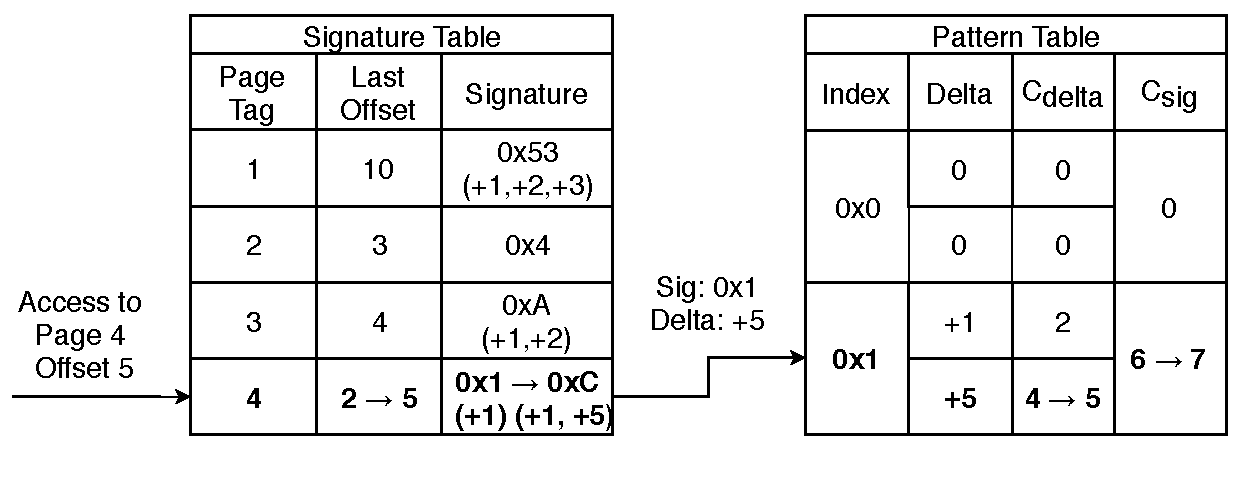
\includegraphics[width=\columnwidth]{SPP_Update_Description}
  \caption{SPP Data-path Flow}
  \label{fig:spp_update}
  \end{center}
\end{figure}


\begin{figure}
  \begin{center}
  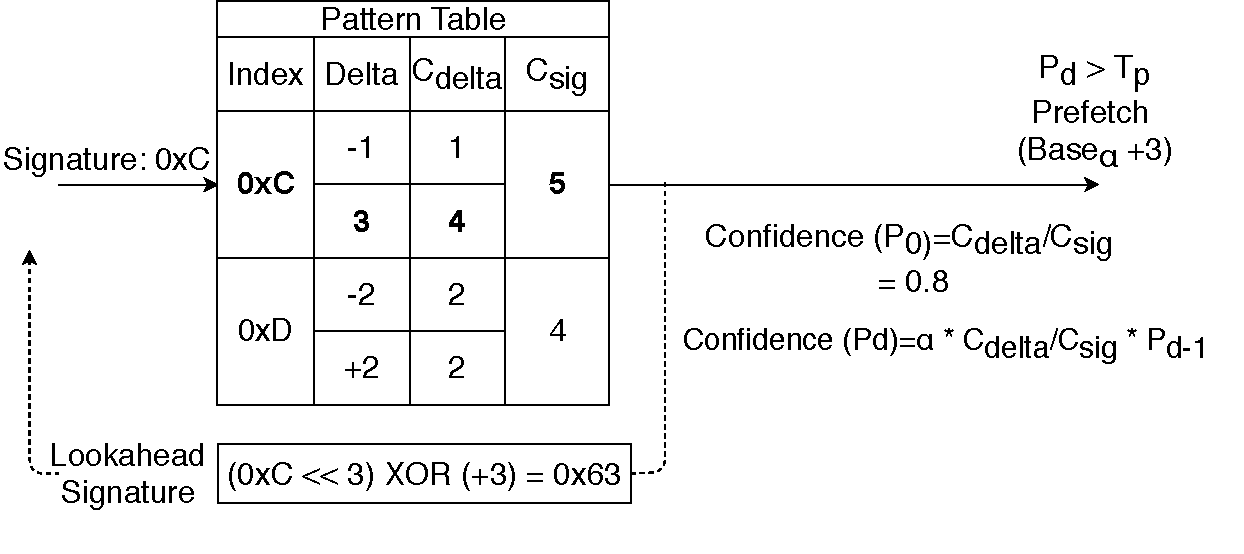
\includegraphics[width=\columnwidth]{SPP_Prefetch_Description}
  \caption{SPP Architecture}
  \label{fig:spp_structure}
  \end{center}
\end{figure}

\subsection{Perceptron Learning}
\label{sec:Background-Perceptron}
Perceptron learning for microarchitectural prediction was introduced
for branch prediction~\cite{PerceptronPredictor}. Our predictor uses a
version of microarchitectural perceptron prediction known as the
``hashed perceptron'' organization~\cite{HashedPerceptron}. As an
abstract idea, a hashed perceptron predictor hashes several different
features into values that index several distinct tables. Small integer
weights are read out from the tables and summed. If the sum exceeds
some threshold, a positive prediction is made, {\em e.g.} ``predict
branch taken'' or ``allow the prefetch.'' Otherwise, a negative
prediction is made. Once the ground truth is known, the weights
corredponding to the prediction are incremented if the outcome was
positive, or decremented if it was negative. This update only occurs
if the prediction was incorrect or if the magnitude of the sum failed
to exceed a threshold.  Beyond branch prediction, perceptron learning
has been applied to last-level cache reuse
prediction~\cite{Perc_Reuse,Multiperspective}. In this paper, we apply
it for doing prefetch filtering.
